% input files

% document's head

\begin{center}
    \LARGE \textsc{Теория к курсу <<Аналитическая механика II>> ФОПФ}
\end{center}

\hrule

\phantom{42}

\begin{flushright}
    \begin{tabular}{rr}
    % written by:
        \textbf{За авторством}: 
        & Хоружего К. \\
        & Примака Е. \\
        &\\
    % date:
        \textbf{От}: &
        \textit{\today}\\
    \end{tabular}
\end{flushright}

\thispagestyle{empty}
\tableofcontents
\newpage

% Lorem ipsum dolor sit amet, consectetur adipisicing elit, sed do eiusmod
tempor incididunt ut labore et dolore magna aliqua. Ut enim ad minim veniam,
quis nostrud exercitation ullamco laboris nisi ut aliquip ex ea commodo
consequat. Duis aute irure dolor in reprehenderit in voluptate velit esse
cillum dolore eu fugiat nulla pariatur. Excepteur sint occaecat cupidatat non
proident, sunt in culpa qui officia deserunt mollit anim id est laborum.
\begin{equation*}
    \vc{\alpha} + \vc{\beta} = \const
\end{equation*}
Lorem ipsum dolor sit amet, consectetur adipisicing elit, sed do eiusmod
tempor incididunt ut labore et dolore magna aliqua. Ut enim ad minim veniam,
quis nostrud exercitation ullamco laboris nisi ut aliquip ex ea commodo
consequat. Duis aute irure dolor in reprehenderit in voluptate velit esse
cillum dolore eu fugiat nulla pariatur. Excepteur sint occaecat cupidatat non
proident, sunt in culpa qui officia deserunt mollit anim id est laborum.


\section{Приближение функций}
\subsection{Протокол BB84}
Пусть есть вертикальная и диагональная поляризация, а также 4 квантовых состояния


шифр Вернама
Протокол Диффи — Хеллмана
Алгоритм RSA

Классическая кирптография: 
    + изученность, стандартизированность
    - не выдерживает создание квантового компьютера

Квантовая криптография:
    + не ставит перехватчик перед вычислительными задачами
    - мало изучены, возможны атаки

Постквантовая криптография:
    + выдерживает существование квантового компьютера
    - недостаточная изученность, авось и классический может взломать


\subsection{Теория Информации}    
пусть $h(p)$ -- информационное содержание события вероятности $p$.
Верно следующее утверждение:
\begin{equation*}
    h(p_1) > h(p_2) \ \ \Leftarrow \ \ p_1 < p_2.
\end{equation*}
Также вполне логично предположить, что $h(1) = 0$, а также что $h(p_1 p_2) = h(p_1)+h(p_2)$. 

Это приводит к функции вида
\begin{equation*}
    h(x) = - \log x = \log_2 \frac{1}{x}
\end{equation*}

\textit{Распределением вероятностей} будем считать некоторый набор $\{p_i\}$ такой, что $\sum p_i = 1$.
Информация, выдаваемая источником может быть найдена, как \textit{матожидание} 
\begin{equation*}
    H(P) = - \sum_i p_i \log p_i,
\end{equation*}
иначе функция называется энтропией Шеннона, -- мера того, насколько неизвестно что выдаст источник. 

Также энтропия Шеннона -- среднее количество вопросов, которые необходимо задать. Ещё это среднее количество битов, которое необходимо, чтобы закодировать выход источника. 

Неравенство Крафта позволяет сформулировать условие к префиксному коду. 

Также можно сформулировать, что разность между практической и теоретической длиной слова $\geq 0$, что соответсвует неравенству Гиббса. 


\begin{itemize}
    \item Коды Хаффмана
    \item Maassen-Uffink entropic
\end{itemize}

\subsection{Измерения в базисе}

Возвращаемся к состояниям 
\begin{align*}
    \cqs{0}{+} &= \qs{0} = \begin{pmatrix}
        1 \\ 0
    \end{pmatrix} \\
    \cqs{1}{+} &= \qs{1} = \begin{pmatrix}
        0 \\ 1
    \end{pmatrix} \\
    \cqs{0}{\times} &= \frac{\qs{0}+\qs{1}}{\sqrt{2}} = \frac{1}{\sqrt{2}} \begin{pmatrix}
        1  \\ 1
    \end{pmatrix} \\
    \cqs{1}{\times} &= \frac{\qs{0}-\qs{1}}{\sqrt{2}} = \frac{1}{\sqrt{2}} \begin{pmatrix}
        1 \\ -1
    \end{pmatrix} \\
\end{align*}
Пусть есть некоторый ортонормированный базис $\{\qs{e_i}\}$ и  состояние $\qs{\xi}$. Вероятность исхода $i$ при измерении $\qs{\xi}$ в базисе $\{\qs{e_i}\}$ равна
\begin{equation*}
    \textnormal{Pr}\, (i) = | \langle e_i | \xi \rangle|^2.
\end{equation*}



\sbsnum{3}{Пространство интегрируемых функций}
\subsubsection*{Неравенства Гёльдера и Минковского}


\begin{to_def}
    \textit{Абсолютно интегрирумыми функциями} на измеримом $X \subseteq \mathbb{R}^n$ называют $f \colon X \mapsto \mathbb{R}$ с конечным интегралом $\int_X |f(x)| \d x$. \textit{Расстоянием}\footnote{
        В силу неравенства $|f(x) - g(x)| \leq |f(x)| + |g(x)|$ расстояние конечно.
    } между функциями $f$ и $g$ будем считать $\int_X |f(x)-g(x)| \d x$.
\end{to_def}

\begin{to_def}
    Обозначим через $L_1 (X)$ факторпространство  линейного пространства абсолютно интегрируемых функций по его линейному подпространству почти всюду равных нулю функций. То есть функции на $0$ расстоянии считаем равными. \textit{Нормой} будем считать
    \begin{equation*}
        \|f\|_1 = \int_X |f(x)| \d x.
    \end{equation*}
\end{to_def}

\begin{to_def}
    Для измеримого по Лебегу $X \subset \mathbb{R}^n$ и числа $p \geq 1$ \textit{факторпространство} измеримых по Лебегу функций на $X$ с конечной (полу)нормой
    \begin{equation*}
        \|f\|_p
        = 
        \left(
            \int_X |f|^p \d x
        \right)^{1/p},
    \end{equation*}
    по модулю функций равных нулю почти всюду,
    назовём $L_p (X)$.
\end{to_def}

\texttt{Очень хорошим, симметричным, актуальным для описания квантовой механики оказывается $L_2$ простран-\\ство, на котором естественно вводить скалярное произведение, его порождающее.} 

 \begin{to_def}
     В комплексном случае норма $L_2$ порождена \textit{скалярным произведением}
     \begin{equation*}
         (f, g) = \int_{-\infty}^{+\infty} f(x) \overline{g(x)} \d x
         \hspace{0.5cm} \longrightarrow \hspace{0.5cm}
         \|f\|_2 = \sqrt{(f, f)}.
     \end{equation*}
 \end{to_def}


\begin{to_thr}[Неравенство Гёльдера]
    Возьмём $p, \, q > 1$ такие, что $1/p + 1/q = 1$. Пусть $f \in L_p (X)$ и $g \in L_q(X)$. Тогда
    \begin{equation*}
        \int_X |fg| \d x \leq \|f\|_p \cdot \|g\|_q.
    \end{equation*}
\end{to_thr}

\begin{proof}[$\triangle$]
    Для доказательства достаточно проинтегрировать неравенство вида
    \begin{equation*}
        |fg| \leq \frac{|f|^p}{p} + \frac{|g|^q}{q}.
    \end{equation*}
    \red{Осталось получить само неравенство.}
\end{proof}

\begin{to_con}
    Для измеримых функций и чисел $p, \, q > 0$, таких что $1/p + 1/q = 1$, имеет место формула
    \begin{equation}
        \label{8_1}
        \|f\|_p = \sup \left\{
            \int_X fg \d x \ \bigg| \  \|g\|_q \leq 1
        \right\}.
    \end{equation}
\end{to_con}


\begin{proof}[$\triangle$]
По неравенству Гёльдера норма $f$ не менее супремума правой части \red{(?)}, более того равенство достигается при выборе
\begin{equation*}
    g(x) = \frac{\sign f(x) |f(x)|^{p-1}}{\|f\|_p^{p-1}}.
\end{equation*}
\end{proof}

\begin{to_def}
    Функция $f \colon V \mapsto \mathbb{R}$ на векторном пространство называется выпуклой, если для любых $x, \, y \in V$ и любого $t \in (0, 1)$ имеет место неравенство
    \begin{equation*}
        f ( (1-t) x + ty) \leq (1-t) f(x) + t f(y).
    \end{equation*}
    Функция называется \textit{строго выпуклой}, если неравенство строгое $\forall x \neq y$ и $t \in (0, 1)$. 
\end{to_def}

\begin{to_lem}
    Если в семействе функций $f_\alpha \colon V \mapsto \mathbb{R}$, $\alpha \in A$, все функции выпуклые, то
    \begin{equation*}
        f(x) = \sup \{f_\alpha (x) \mid \alpha \in A\}
    \end{equation*}
    тоже выпуклая\footnote{
        Если разрешить в определении выпуклости значение $+ \infty$.
    }.
\end{to_lem}


\begin{to_thr}[Неравенство Минковского]
    Для функций $f, \, g \in L_p$ при $p \geq 1$
    \begin{equation*}
        \|f + g\|_p \leq \|f\|_p + \|g\|_p.
    \end{equation*}
\end{to_thr}



\subsubsection*{Полнота пространства интегрируемых функций}

Далее в разделе всегда предполагается суммирование по $k$ от $1$ до $\infty$. Глобально можно сказать, что \texttt{в нормированном пространстве вопрос полноты сводится в вопросу сходимости рядов}, у которых сходятся суммы норм. 

\begin{to_def}
    Назовём последовательность $(f_n)$ \textit{фундаментальной}, если
    \begin{equation*}
        \forall \varepsilon > 0 \ 
        \exists N_\varepsilon \colon 
        \forall n, m \geq N_\varepsilon \
        \|f_n - f_m\|_p < \varepsilon.
    \end{equation*}
\end{to_def}

\begin{to_lem}
    Пусть у последовательности функций $(u_k)$ из $L_p (X)$ сумма
    $\sum \|u_k\|_p$
    оказалась конечной. Тогда $S(x) = \sum u_k (x)$ определена для почти всех $x$ и
    $\|S\|_p \leq \sum \|u_k\|_p.$
\end{to_lem}


\begin{to_lem}
    Пусть у последовательности функций $(u_k)$ из $L_p (x)$ сумма
    $\sum \|u_k\|_p$
    оказалась конечной. Тогда $S(x) = \sum u_k (x)$ определена для почти всех $x$ и
    $S = \sum u_k$
    в смысле сходимости в пространстве $L_p (X)$.
\end{to_lem}


\begin{to_thr}[]
    Пространство $L_p (X)$ полно.
\end{to_thr}



Вообще сходимость в $L_p (X)$ может не означать поточечной сходимости ни в одной точке.

\sbsnum{4}{Приближение функций ступенчатыми и бесконечно гладкими}
\section{Интерференция}


\subsection{Конечные размеры источника и пространственная когерентность}


\textbf{Два точечных источника}.
Рассмотрим интереференцию света от двух источников $A$ и $B$ (рис. \eqref{fig281}). 
\begin{figure}[ht]
    \centering
    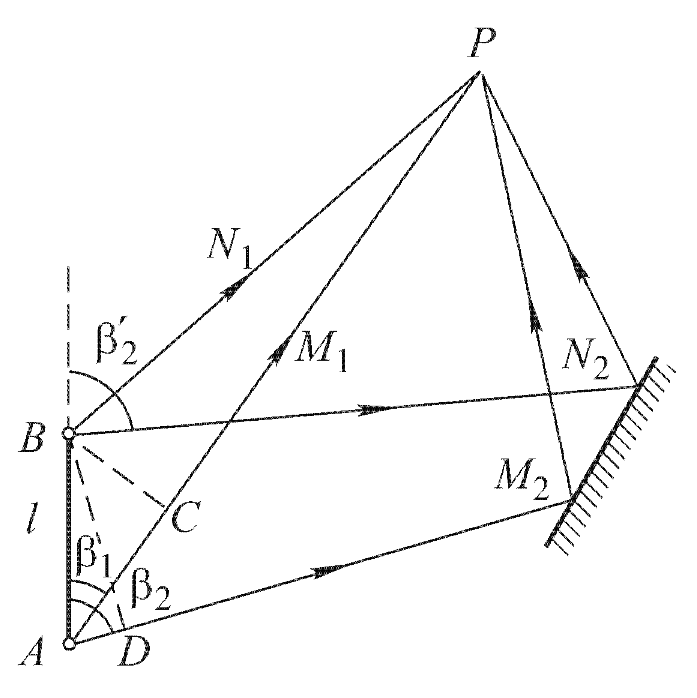
\includegraphics[width=0.3\textwidth]{figures/28_1.png}
    \hspace{5 mm} 
    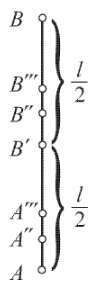
\includegraphics[width=0.09\textwidth]{figures/28_2.png}
    \caption{К пространственной когерентности}
    \label{fig281}
\end{figure}
Считая $l=AB$ достаточно малым, то для разности оптических лучей можно написать $l\cos \beta_1$ и $l \cos \beta_2$. Тогда для разности оптической разности хода лучей от $A$ и $B$ верно, что
\begin{equation*}
    \Delta = 
    \left[(AM_1P)-(AM_2P)\right]-\left[(BN_1 P) - (BN_2P)\right]
   = l |\cos \beta_1 - \cos \beta_2|,
\end{equation*}
которая определяет сдвиг одной интерфереционной картины относительно другой. При $\Delta = \lambda/2$ максимумы одной -- минимумы другой, при $\Delta = \lambda$ резонируют. 

Стоит заметить, что мы условно считаем, что при $\Delta = (m+1/4)\lambda,\, m \in \mathbb{Z}$ -- всё хорошо. А ещё $\beta = \beta'$. 



\textbf{Протяженный источник}.  Считая, что все точки излучают некогерентно, разобьём на пары источников $(A, B'),\,  (A'', B'')$ и т.д. находящиъся на $l/2$ друг от друга. Тогда, при $\Delta/2 = \lambda/2$ от каждой пары будет просто светлый фон, получаем условия
\begin{equation*}
    \Delta \equiv l(\cos \beta_2 - \cos \beta_2) = m\lambda,
\end{equation*}
при выполнении которого на экране один только освещенный фон без полос. При $\Delta = (m+\alpha)\lambda$ источник можно разбить на две части $m \colon  \alpha$, где меньшая часть источника даст интерференционные полосы на светлом фоне от большей части источника. 

Если крайние лучи выходят симметрично к $\bot AB$, т.е. $\beta_2 = \pi-\beta_1$, то $\cos \beta_2 = - \cos \beta_1$, и тогда хорошая интерференция будет при
\begin{equation*}
    (l/2) |\cos\beta_1-\cos \beta_2| \leq \lambda/4,
    \hspace{10 mm} 
    l \sin (\Omega/2) \leq \lambda/4,
\end{equation*}
где $\Omega$ -- угол между крайними лучами, угол интерференциии. 


\begin{to_def}
    Два источника, позволяющие наблюдать интереференцию света от них, называют \textit{пространственно когерентными}, иначе -- \textit{пространственно некогерентными}. 
\end{to_def}

В случае же монохроматичного света, можем говорить про пространственную когерентность при 
\begin{equation*}
    \sigma =\pi \lambda^2 / (4 \varphi^2). 
\end{equation*}

Рассмотри два точечных немонохроматичных источников света: длины волн $\lambda$ и $\lambda' = \lambda+\delta \lambda$. Точка с $\Delta = 0$ -- \textit{центр интерференионной картины}. 

\textbf{Две спектральные линии}. Если фазы $S_1$ и $S_2$ то центр сохранится. Волны придут в противофазе, при
\begin{equation*}
    N \lambda' = \left(N + \frc{1}{2}\right) \lambda,
    \hspace{0.5cm} \Rightarrow \hspace{0.5cm}
    N = \frac{\lambda}{2(\lambda'-\lambda)} = \frac{\lambda}{2 \delta \lambda}.
\end{equation*}
Когда номер полосы мал по сравнению с величиной $N$, интерференционные полосы будут отчётливы, при номере $N$ для $\lambda$ и $(N+1.2)$ для $\lambda'$ полосы пропадут, а вот на $2N$ и $2N+1$ уже снова будут в фазе.

\textbf{Кусочек спектра}. Пусть теперь $\lambda \in (\lambda,\,  \lambda+\delta \lambda)$, тогда разобьём всё на пары на расстоянии $\delta \lambda/2$ друг от друга, к каждой из которых верно значение для $N$ (при $\delta \lambda \to \delta \lambda/2$), поэтому первые полосы исчезнут при
\begin{equation*}
    N = \lambda / \delta \lambda,
\end{equation*}
что в два раза больше дискретного случая. 



\textbf{Временная когерентность}.
Вообще можно сказать, что для когерентности необходимо, чтобы разность хода лучей не превосходила длину цуга $L = c \tau$,  тогда
\begin{equation*}
    \sub{N}{max} = \frac{L}{\lambda} = \frac{\tau}{T} = \frac{\lambda}{\delta \lambda} = \frac{\omega}{\delta \omega}.
\end{equation*}
Если учесть, что $\lambda = 2\pi / k$ и $T = 2 \pi/\omega$, то $\tau \cdot \delta \omega = 2 \pi$ и $L \cdot \delta k = 2 \pi$. 

Так как здесь основной игрок -- длина цуга, то говорят про \textit{пространственную когерентность}, связанная с \textit{узостью спектрального интервала} $\Delta \omega$. Для времени когерентности верно соотношение
\begin{equation*}
    \sub{\tau}{ког} \approx \frac{2\pi}{\Delta \omega} \approx \frac{1}{\Delta \nu},
    \hspace{0.5cm} \Rightarrow \hspace{0.5cm}
    L \approx c \sub{\tau}{ког} = \lambda \frac{\nu}{\delta \nu} = \frac{\lambda^2}{\delta \lambda},
\end{equation*}
что называется \textit{длиной когерентности}.








\textbf{Квазимонохроматичность}. 
Если область $\Delta \omega$ в которую входит 
% $p.\, v.$
 основное значение интеграла Фурье, и $\Delta \omega / \omega \ll 1$, то результирующее колебание называется \textit{квазимонохроматическое}. Запишем произвольные квазимонохроматические колебания в виде
\begin{equation*}
    E(t) = a(t) e^{i \omega_0 t},
\end{equation*}
где $a(t)$ -- медленная амплитуда, таким образом колебания модулированы, меняется $a(t)$ -- амплитудная модуляция, меняется фаза -- \textit{фазовая модуляция}. 


Так как детекция происходит в основном для интенсивности, то про неё и будем гворить, квадрат поля может быть представлен в виде
\begin{equation*}
    (\Re E)^2 = \left(\frac{E + E^*}{2}\right)^2 = \frac{1}{4} \left(E^2 + E^{*2}\right) + \frac{1}{2} E E^*.
\end{equation*}
Если считать $a = a_0 (t) e^{i \delta(t)}$, где $a_0(t)$ и $\delta(t)$ -- межденно меняющиеся вещественная амплитуда и фаза, то
\begin{equation*}
    E^2 + E^{*2} = 2 a_0^2 \cos\left[2(\omega_0 r + \delta)\right],
\end{equation*}
что быстроосциллирует, так что $0$. Поэтому интенсивность $\langle E E^*\rangle$. 



\textbf{Два источника}.
Рассмотрим теперь сумму колебаний от двух источников из $S_1$ и $S_2$ с отставваиями на $\theta_1$ и $\theta_2$. Тогда результирующее 
\begin{equation*}
    E \equiv E(P, t) = E_1(t-\theta_1) + E_2 (t-\theta_2).
\end{equation*}
Умножая на комплексно-сопряженное и усредняя по времени приходим к выражению вида
\begin{equation*}
    I = I_1 + I_2 + 2 \sqrt{I_1 I_2} \Re\left[f_{12}(\theta)\right],
\end{equation*}
где $\theta = \theta_2-\theta_1$. 

\begin{to_def}
    \textit{Корреляционной функцией} колебаний $E_1(t-\theta_1)$ и $E_2(t-\theta_2)$ называют 
    \begin{equation*}
        \left\langle 
            E_1(t-\theta_1) E_2^* (t-\theta_2)
        \right\rangle = \left\langle E_1(t) E_2^* (t-\theta)\right\rangle = F_{1, 2}(\theta) = \sqrt{I_1 I_2}f_{1,2} (\theta).
    \end{equation*}
    Она характеризует степень согласованности колебаний. Функция $f_{1, 2}$ называется \textit{нормированной корреляционной функцией}. Разделив её на быстро осциллирующую функцию $e^{i \omega_0 t}$ можем перейти к \textit{комплексной степени когерености колебаний}
    \begin{equation*}
        \gamma_{1,2}(\theta) = f_{1, 2} (\theta) e^{-i \omega_0 \theta},
    \end{equation*}
    модуль которой -- степень когерентнсоти колебаний в точке $P$. 
\end{to_def}



Итого, в терминах $\gamma$, переходим к
\begin{equation*}
    I = I_1 + I_2 + 2 \sqrt{I_1 I_2} \Re\left[\gamma(\theta) e^{i \omega_0 \theta}\right] = 
    I_1 + I_2 + 2 \sqrt{I_1 I_2}  |\gamma_{1,2}(\theta)| \cos(\omega_0 \theta + \delta(\theta)),
\end{equation*}
где $\gamma_{1,2} (\theta) = |\gamma_{1, 2}|e^{i \delta}$. Однако $\gamma$ меняется медленно, так что в максимумах $\cos(\omega_0 \theta + \delta) = +1$ и в минимумах $\cos(\omega_0 \theta + \delta) = -1$, тогда
\begin{equation*}
    \sub{I}{max} = I_1 + I_2 + 2 \sqrt{I_1 I_2} |\gamma_{1, 2} (\theta)|,
    \hspace{5 mm} 
    \sub{I}{min} = I_1 + I_2 - 2 \sqrt{I_1 I_2} |\gamma_{1, 2} (\theta)|,
    \hspace{0.5cm} \Rightarrow \hspace{0.5cm}
    V \equiv \frac{\sub{I}{max}-\sub{I}{min}}{\sub{I}{max}+\sub{I}{min}} = \frac{2 \sqrt{I_1 I_2}}{I_1 + I_2} |\gamma_{1,2} (\theta)|.
\end{equation*}
Получается, что при $\gamma_{1, 2}(\theta) =0$ колеабния \textit{некогеренты}, и если $\gamma_{1, 2}(\theta) \equiv 0,\, \forall \theta$, то \textit{некогерентность полная}, тогда всюду имеет место \textit{закон фотометрического сложения}. 

Интереференция \textit{полная} при $\gamma_{1, 2}(\theta) \equiv 1$, такой случай реализуется при наложении строго
периодических, в частности монохроматических, пучков одинаковых периодов. Вопросы \textit{пространственной} и \textit{временной} когерентности колебаний некоторого поля могут быть сведены к рассмотрению $\gamma$ для ситуции рис. \ref{fig:31}.
\begin{figure}[h]
    \centering
    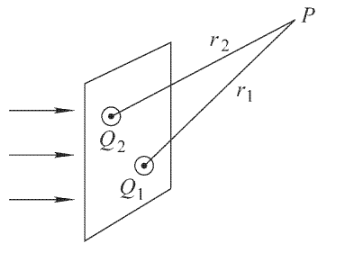
\includegraphics[width=0.27\textwidth]{figures/31_1.png}
    \caption{Расчёт пространственной и временной когерентности.}
    \label{fig:31}
\end{figure}


\textbf{Оборванная синусоида}. Пусть есть $\sin$ вплоть до некоторого $\tau$ по которому и будем усреднять
\begin{equation*}
    E(t) = \left\{\begin{aligned}
        &\sin \omega_0 t, &t \in[0, \tau], \\
        &0,     &t \notin [0, \tau],
    \end{aligned}\right.
    \hspace{0.5cm} \Rightarrow \hspace{0.5cm}
    \gamma(\theta) = \left\{\begin{aligned}
        &1-\theta/\tau, &\theta < \tau, \\
        &0, &\theta > \tau.
    \end{aligned}\right.
\end{equation*}
что может быть получено из выражения
\begin{equation*}
    \left\langle E(t) E^* (t-\theta)\right\rangle = \frac{1}{\tau} \int_0^\tau e^{i \omega_0 \theta} \d t = \frac{\tau-\theta}{\tau} e^{i \omega_0 \theta} = F(\theta) = f(\theta).
\end{equation*}


\textbf{Связь автокорреляционной функции и спектральной плотности}. Да, они связаны: $F(\theta)$ и $I_\omega(\omega)$. Для установления связи запишем по определению
\begin{equation*}
    F(\theta) = \left\langle E(t) E^* (t-\theta)\right\rangle = \frac{1}{\tau} \int_{-\tau/2}^{\tau/2} E(t) E^* (t-\theta) \d t,
\end{equation*}
подтсавляя $E^*(t-\theta) = \int_0^\infty a^* (\omega) e^{-i \omega (t-\theta)} \d \omega$, а также вспоминая выражения для $a(\omega)$, и меняя порядок интегрирования приходим к
\begin{equation*}
    a(\omega) = \frac{1}{2\pi} \int_{-\tau/2}^{\tau/2} E(t) e^{-i \omega t} \d t,
    \hspace{0.5cm} \Rightarrow \hspace{0.5cm}
    F(\theta) = \frac{2\pi}{\tau} \int_{0}^{+\infty}  a^*(\omega) a(\omega) e^{i \omega \theta} \d \omega = 
    \int_{0}^{\infty} I_\omega (\omega) e^{i \omega \theta} \d \omega,
\end{equation*}
где учтено, что $I_\omega (\omega) = \frac{2\pi}{\tau} a^*(\omega) a(\omega)$. Это формула -- фурье-разложение $F(\theta)$, поэтому верно и обратное
\begin{equation*}
    F(\theta) = \int_{0}^{\infty} I_\omega (\omega) e^{i \omega \theta} \d \omega,
    \hspace{0.5cm} \Rightarrow \hspace{0.5cm}
    I_\omega (\omega) = \frac{1}{2\pi} \int_{-\infty}^{+\infty} F(\theta) e^{-i \omega \theta} \d \theta.
\end{equation*}
Вообще можно показать, что $F(-\theta) = F^*(\theta)$, тогда последняя формула перепишется в виде:

\begin{to_thr}[теорема Винера-Хинчина]
    Связь между спектральной плотностью мощности сигнала и его автокорреляционной функцией может быть записана в виде:
    \begin{equation*}
    I_\omega (\omega) = \frac{1}{2\pi}\left[
        \int_{0}^{\infty} F(\theta) e^{- i \omega \theta} \d \theta + \text{c.c.}
    \right],
    \end{equation*}
    что позволяет измерять $I_\omega$ для волн.
\end{to_thr}

% Так можно мерять $I_\omega$!
\subsection{Теорема Ван-Циттера-Цернике}

Пространственную когерентность $\gamma_{1, 2}$ для точек $Q_1$ и $Q_2$ экрана, освещаемого протяженным квазимонохроматическим самосветящимся источником света. Если рассматриваемая точка $P$ равноудалена от $Q_1$ и $Q_2$ то можем рассматривать просто волны в $Q_1$ и $Q_2$. В качетсве источника рассматривается площадка $\sigma$ $\parallel$ экрану. 


В точках $Q_1$ и $Q_2$ может быть определена интенсивность
\begin{equation*}
    I_1 \equiv I(Q_1) = \int_\sigma \frac{I(S) \d S}{r_1^2}, \hspace{5 mm} 
    I_2 \equiv I(Q_2) = \int_\sigma \frac{I(S) \d S}{r_2^2}.
\end{equation*}
Введя нормирующий множитель, можем найти $\gamma_{1,2} (\theta \ll 1)$:
\begin{equation*}
    \gamma_{1,2} (0) = \frac{1}{\sqrt{I_1 I_2}} \int \frac{I(S)}{r_1 r_2} e^{ik (r_2-r_1)} \d S.
\end{equation*}
Таким образом мы говорим, что:

\begin{to_thr}[теорема Ван-Циттера-Цернике]
    Комплексная степень взаимной когерентности в точках $Q_1$ и $Q_2$ равна комплексной амплитуде в точке $Q_1$ соответстствующей дифрагированной волны.
\end{to_thr}





\section{Ограниченная вариация, абсолютная непрерывность и осцилляция}
\sbsnum{5}{Функции ограниченной вариации}
\begin{to_def}
    Функция $f$ на промежутке $I$ имеет \textit{ограниченную вариацию}, если для любых $x_0 < x_1 < \ldots M x_N \in I$ (в любом количестве)
    \begin{equation*}
        |f(x_0) - f(x_1)| + 
        |f(x_1) - f(x_2)| + \ldots +
        |f(x_{N-1}) - f(x_N)| \leq M,
    \end{equation*}
    для некоторой константы $M$. Наименьшую константу $M$ в этом неравенстве назовём вариацией функции $f$ равную $\|f\|_B$, что задаёт \textit{полунормой}.
\end{to_def}


\begin{to_lem}
    Функцию ограниченной вариации на отрезке $[a, b]$ можно представить в виде суммы двух функций $f = u + d$, одна из которых возрастает, а другая убывает. При этом $\|f\|_B = \|u\|_B + \|d\|_B$ и если $f$ была непрерывной, то $u$ и $d$ тоже будут непрерывны.
\end{to_lem}


\red{Дополнить смыслом функций с ограниченной вариацией.}

\sbsnum{6}{Абсолютно непрерывные функции и обобщенная формула Ньютона-Лейбница}
Для формулы Ньютона-Лейбница условие липшицевости можно ослабить до следующего:

\begin{to_def}
    Функция $F$ на промежутке $I$ \textit{абсолютно непрерывна} , если $\forall \varepsilon > 0 \ \exists \delta_\varepsilon > 0$, такое что
    $\forall \, x_1 \leq y_1 \leq x_2 \leq y_2 \leq \ldots \leq x_N \leq y_N \in I$ из неравенства
    \begin{equation*}
        |x_1 - y_1| + |x_2 - y_2| + \ldots + |x_N - y_N| \leq \delta
    \end{equation*}
    следует, что
    \begin{equation*}
        |F(x_1)-F(y_1)| + 
        |F(x_2)-F(y_2)| + 
        \ldots +
        |F(x_N)-F(y_N)| \leq \varepsilon.
    \end{equation*}
    \texttt{
    Говоря неформально, сумма модулей приращений функции на системе непересекающихся отрезков должна \\ стремиться к нулю при суммарной длине системы, стремящейся к нулю.
    } 
\end{to_def}

\begin{to_lem}
    
\end{to_lem}


\begin{to_thr}[]
    Для некоторой $f \in L_1 [a, b]$, всякая обобщенная первообразная $F$ 
    \begin{equation*}
        F(x) = \int_a^x f(t) \d t,
    \end{equation*}
     является абсолютно непрерывной и её производная почти всюду существует и совпадает с $f$.
\end{to_thr}


\begin{to_lem}
    Абсолютно непрерывная на отрезке функция $f$ имеет на нём ограниченную вариацию. Также на отрезке существует разложение $f$ в сумму двух монотонных абсолютно непрерывных функций.
\end{to_lem}


\begin{to_thr}[]
    Абсолютно непрерывная функция $F \colon [a, b] \mapsto \mathbb{R}$ почти всюду имеет производную и является обобщенной первообразной своей производной с выполнением формулы Ньютона-Лейбница
    \begin{equation*}
        F(b) - F(a) = \int_a^b F' (t) \d t.
    \end{equation*}
\end{to_thr}

\red{Легко показать через\ldots ух, ну по \textbf{лемме Безиковича}, посмотреть можно
\href{https://youtu.be/kTzJlaSrK7Y?list=PLthfp5exSWErwR6-3PMFN9w_iGJBdlXfZ&t=4030}{здесь}.}

\begin{to_con}[Обобщенное интегрирование по частям]
    Если $f \in L_1 [a, b]$, а $g$ абсолютно непрерывна, то верна формула интегрирования по частям
    \begin{equation*}
        \int_a^b f g \d x = F(x) g(x) \bigg|_a^b
        - \int_a^b F(x) g'(x) \d x,
    \end{equation*}
    где $F(x) = \int_a^x f(t) \d t$.
\end{to_con}


\begin{to_lem}
    Функция $f \colon [a, b] \mapsto \mathbb{R}$ абсолютно непрерывна тогда и только тогда, когда она может быть сколь угодно близко в $B$-норме приближена кусочно-линейными функциями.
\end{to_lem}

\red{А дальше про борелевские меры на отрезках и интеграл Лебега–Стилтьеса.}



\sbsnum{7}{(до 2.9) Осцилляции и равномерные осцилляции}
\begin{to_def}
    Определим \textit{коэффициент Фурье} (с точностью до умножения на константу)
    \begin{equation*}
        c_f (y) = \int_{-\infty}^{+\infty} f(x) e^{-ixy} \d x.
    \end{equation*}
\end{to_def}

\begin{to_thr}[]
    Если $f \in L_1 (\mathbb{R})$, то $|c_f (y)| \leq \|f\|_1$ и $c_f (y)$ непрерывно зависит от $y$.
\end{to_thr}

\begin{to_thr}[Лемма об осцилляции]
    Если $f \in L_1 (\mathbb{R})$, то выражение
    \begin{equation*}
        c_f (y) = \int_{-\infty}^{+\infty} f(x) e^{-ixy} \d x
    \end{equation*}
    стремится к нулю при $y \to \infty$.
\end{to_thr}

\begin{to_lem}
    Еси производная $f^{(k-1)}$ абсолютно непрерывна и производные до $k$-й включительно\footnote{
        Для $k$-й достаточно существования почти всюду.
    }  находятся в $L_1 (\mathbb{R})$, то
    \begin{equation*}
        c_f (y) = o \left(\frac{1}{y^k}\right),
        \hspace{1 cm}
        t \to \infty.
    \end{equation*}
\end{to_lem}

\begin{to_thr}[]
    Если $f \in L-1 (\mathbb{R})$ имеет ограниченную вариацию на $\mathbb{R}$, то выражение
    \begin{equation*}
        c_f (y) = \int_{-\infty}^{+\infty} f(x) e^{-ixy} \d x
    \end{equation*}
    оказывается $O(1/y)$ при $y \to \infty$.
\end{to_thr}

\begin{to_con}
    Пусть функция $f \colon \mathbb{R} \mapsto \mathbb{R}$ имеет абсолютно непрерывную $(k-1)$-ую производную, производные до $k$-й включительно находятся в $L_1 (\mathbb{R})$, а $f^{(k)}$ (возможно, после изменения на множестве меры нуль) имеет ограниченную вариацию на $\mathbb{R}$, тогда
    \begin{equation*}
        c_f (y) = \int_{-\infty}^{+\infty} 
        f(x) e^{-ixy} \d x =
        O\left(\frac{1}{y^{k+1}}\right), 
        \hspace{1 cm}
        y \to \infty.
    \end{equation*}
\end{to_con}



\begin{to_thr}[Лемма о равномерной осцилляции]
    Если $f \in L_1(\mathbb{R})$, то выражение
    \begin{equation*}
        c(y, \xi, \eta) = \int_\xi^\eta f(x) e^{-ixy} \d x
    \end{equation*}
    стремится к нулю при $y \to \infty$ равномерно по $\xi, \ \eta$.
\end{to_thr}


\subsubsection*{Периодические функции}


\begin{to_def}
    Для $2\pi$-\textit{периодической функции}  $f(x+2\pi) \equiv f(x)$ \textit{коэффициенты Фурье}  запишутся, как
    \begin{equation*}
        c_n = \frac{1}{2\pi} \int_{-\pi}^{\pi} 
        f(x) e^{-inx} \d x = 
        \frac{
        (f, e^{inx})
        }{
        \|e^{inx}\|_2^2
        },
    \end{equation*}
    где последнее выражение понимается в смысле скалярного произведения и нормы в $L_2 [-\pi, \pi]$.
\end{to_def}

\begin{to_thr}[]
    Пусть функция $f$ имеет период $2 \pi$ и абсолютно непрерывную $(k-1)$-ую производную, причём $f^(k)$ (возможно, после изменения на множестве меры нуль) имеет ограниченную вариацию на $[-\pi, \pi]$, тогда
    \begin{equation*}
        c_n = \frac{1}{2\pi} \int_{-\pi}^{\pi} f(x) e^{inx} \d x =
        O\left(\frac{1}{n^{k+1}}\right),
        \hspace{1 cm}
        n \to \infty.
    \end{equation*}
\end{to_thr}


\begin{to_lem}
    Усли у $2\pi$-периодической функции ограниченной вариации есть ненулевое конечное число разрывов, и она кусочно абсолютно непрерывна, то оценка $O(1/n)$ для коэффициентов Фурье неулучшаема.
\end{to_lem}

\begin{to_thr}[]
    Пусть функция $f$ непрерывна и $2\pi$-периодическая, тогда для коэффициента Фурье имеется оценка
    \begin{equation*}
        c_n = O(\omega_f (\pi/n)),
    \end{equation*}
    где $\omega_f$ -- модуль непрерывности $f$.
\end{to_thr}


\section{Ряд Фурье в пространстве \texorpdfstring{$L_2$}{L2}}
\begin{to_thr}[Теорема Вейерштрасса для тригонометрических многочленов]
    \label{thr_4.77}
    Всякую непрерывную на $[-\pi, \pi]$ функцию $f$, для которой $f(-\pi)=f(\pi)$, можно сколь угодно близко равномерно приблизить тригонометрическими многочленами вида
    \begin{equation*}
        T(x) = a_0 + \sum_{k=1}^{n} (a_k \cos kx + b_k \sin kx).
    \end{equation*}
\end{to_thr}

\begin{to_thr}[Теорема Стоуна-Вейерштрасса]
    Пусть у нас зафиксирован компакт $K$ и дана алгебра непрерывных функций $\mathcal A$ на этом компакте, которая разделяет точки, то есть для любых $x \neq y \in K$ найдётся $f \in \mathcal A$, такая что $f(x) \neq f(y)$. Тогда Всякую непрерывную на $K$ функцию можно сколь угодно близко равномерно приблизить функциями из $\mathcal A$.
\end{to_thr}

\red{Вспомнить про $\|f\|_C$.} Равномерное приближение является приближением по норме $L_2$, так как на отрезке $[-\pi, \pi]$ имеется неравенство $\|f\|_2 \leq \sqrt{2\pi} \|f\|_C$. В случае $L_2$ нормы определим коэффициенты, которыми собираемся приближать.

\begin{to_thr}[Оптимальность коэффициентов Фурье]
    Для всякой $f \in L_2[-\pi, \pi]$ и данного числа $n$ лучшее по норме $L_2$ приближение $f$ тригонометрическим многочленом $\sum_{-n}^{+n} c_k e^{ikx}$ дают коэффициенты Фурье
    \begin{equation*}
        c_k = \frac{1}{2\pi} \int_{-\pi}^{\pi} f(x) e^{ikx} \d x.
    \end{equation*}
\end{to_thr}


\begin{to_lem}[неравенство Бесселя]
    Из доказательства предыдущей теоремы, можем получить, что
    \begin{equation*}
        \left\|f - \sum_{k=1}^N c_k \varphi_k \right\|_2^2 = 
        \|f\|_2^2 - \sum_{k=1}^{N} |c_k|^2 \|\varphi_k\|_2^2,
        \hspace{0.7 cm} \Rightarrow \hspace{0.7   cm}
        \|f\|_2^2 \geq  \sum_{k=1}^{\infty} |c_k|^2 \|\varphi_k\|^2_2,
        \hspace{0.5cm} \overset{\mathrm{trig}}{\Rightarrow}  \hspace{0.5cm}
        \|f\|_2^2 \geq 2\pi \sum_{k=-n}^n |c_k|^2.
    \end{equation*}
    \red{Точно ли до $n$?}
\end{to_lem}

\begin{to_lem}[Представление действительнозначной функции]
    Для действительнозначной функции представление в виде ряда Фурье перепишется в виде
    \begin{equation*}
        f = \sum_{k=0}^{n} (a_k \cos kx + b_k \sin kx),
        \hspace{1 cm}
        a_k = \frac{1}{\pi}\int_{-\pi}^{\pi} f(x) \cos kx \d x,
        \hspace{0.5 cm}
        b_k = \frac{1}{\pi} \int_{-\pi}^{\pi} f(x) \sin kx \d x,
    \end{equation*}
    для $k \geq 1$. Неравенство Бесселя тогда запишется так:
    \begin{equation*}
        \|f\|_2^2 \geq \frac{\pi}{2} |a_0|^2 + 
        \pi \sum_{k=1}^{\infty} (|a_k|^2 + |b_k|^2).
    \end{equation*}
\end{to_lem}

\begin{to_thr}[Сходимость ряда Фурье в среднеквадратичном]
    Для вской комплекснозначной $f \in L_2 [-\pi, \pi]$
    \begin{equation*}
        f = \sum_{k=-\infty}^{\infty} 
        c_k e^{ikx} = 
        \lim_{n \to \infty} \sum_{k=-n}^{n} c_k e^{ikx}
    \end{equation*}
    в смысле сходимости суммы в пространстве $L_2[-\pi, \pi]$, а также выполняется равенство Парсеваля
    \begin{equation*}
        \|f\|_2^2 = 2 \pi \sum_{k=-\infty}^{\infty} |c_k|^2.
    \end{equation*}
\end{to_thr}

\texttt{Пока мы не доказали, что в полученную формулу можно подставить хоть одно конкретное значение $x$. Тот факт, что ряд Фурье функции из
$L_2[-\pi, \pi]$ на самом деле сходится к этой функции почти всюду, был доказан Л. Карлесоном (1966), а до этого был известен как гипотеза Лузина.} 


\section{Ряд Фурье и его сходимость}
\begin{to_def}
    Обозначим \textit{частичную сумму} тригонометрического ряда Фурье для $2\pi$-периодической функции $f$ как
    \begin{equation*}
        T_n (f, x) = \sum_{k=-n}^n c_k (f) e^{ikx}.
    \end{equation*}
\end{to_def}

\begin{to_lem}
    Для $n$-й частичной суммы ряда Фурье $2\pi$-периодической функции имеет место формула в виде свёртки
    \begin{equation*}
        T_n (f, x) = \int_{-\pi}^{\pi} f(x+t) D_n (t) \d T,
    \end{equation*}
    с ядром Дирихле
    \begin{equation*}
        D_n (t) = \frac{1}{2\pi} \frac{\sin \big(\left(n+\frac{1}{2}\right) t\big)}{\sin\left(\frac{1}{2} t\right)}.
    \end{equation*}
\end{to_lem}


\begin{to_lem}[Равномерная ограниченность интегралов от ядра Дирихле]
    Существует такая константа $C$, что 
    \begin{equation*}
        \left|
        \int_a^b D_n (t) \d t
        \right| \leq C
    \end{equation*}
    для любых $a, b \in [-\pi, \pi], \ n \in \mathbb{N}$.
\end{to_lem}

\begin{to_thr}[Равномерный принцип локализации]
    Запищем для $\delta \in (0, \pi)$
    \begin{equation*}
        T_n (f, x) - f(x) = 
        \int_{-\pi}^{\pi} 
        \left(
            f(x+t) - f(x)
        \right) D_n (t) \d t =
        \int_{-\delta}^{\delta} \left(
            f(x+t) - f(x)
        \right) D_n (t) \d t + 
        \int_M 
        (f(x+t)-f(x)) D_n (t) \d t,
    \end{equation*}
    где $M = \left\{t \mid \delta \leq |t| \leq \pi\right\}$. Если $f \in L_1 [-\pi, \pi]$, то
    \begin{equation*}
        \int_M \left(
            f(x+t) - f(x)
        \right) D_n (t) \d t
        \ \to \ 0, \hspace{0.5 cm} n \to \infty.
    \end{equation*}
    Если $f$ ограничена на отрезке $[a, b]$, то это выражение стремится к нулю равномерно по $x \in [a, b]$.
\end{to_thr}


\begin{to_def}
    Функция $f$ называется гёльдеровой степени $\alpha > 0$, если для любых $x, \, y$ из области определения
    \begin{equation*}
        |f(x) -f(y)| \leq C |x-y|^{\alpha}
    \end{equation*}
    с некоторой константой $C$.
\end{to_def}


\begin{to_thr}[Признак Липшица сходимости ряда Фурье]
    Для абсолютно интегрируемой $2\pi$-периодической функции, которая является гёльдеровой с некоторыми $C$, $\alpha > 0$ на интервале $(A, B) \supset [a, b]$
    \begin{equation*}
        T_n (f, x) \to f(x)
    \end{equation*}
    равномерно $x \in [a, b]$ при $n \to \infty$.
\end{to_thr}

\begin{to_thr}[Признак Дирихле сходимости ряда Фурье]
    Для абсолютно интегрируемой $2\pi$-периодической функции, которая является непрерывной с ограниченной вариацией на интервале $(A, B) \supset [a, b]$
    \begin{equation*}
        T_n (f, x) \to f(x)
    \end{equation*}
    равномерно по $x \in [a, b]$ при $n \to \infty$.
\end{to_thr}

\red{Далее несколько лемм, сформулированных в виде задач, а именно признак Дирихле сходимости ряда Фурье в точке, признак Липшица сходимости ряда Фурье в точке, признак Дини сходимости ряда Фурье в точке. Ага, это 13 тема. А потом будут темы 14 - 17.}





% \begin{equation*}
%     f \colon  X \to Y
% \end{equation*}
\newpage
\section*{Собственные интегралы с параметром}


\subsection*{13.8(3)}


Стоит следующий вопрос
\begin{equation*}
    \int_0^1 \d x \int_0^1 \d \alpha f(x, \alpha) - \int_0^1 \d \alpha \int_0^1 \d x f(x, \alpha) \overset{?}{=} 0.
\end{equation*}
Выберем в качестве $f(x, \alpha)$ 
\begin{equation*}
    f(x, \alpha) = \left(
        \frac{x^5}{\alpha^4} - \frac{2 x^3}{\alpha^3}
    \right) e^{-x^2/\alpha}.
\end{equation*}
Для этого вычислим интеграл
\begin{equation*}
    g(x) = \int_0^1 \d \alpha f(x, \alpha) = \int_0^1 \d \alpha \left(
        \frac{x^5}{\alpha^4} - \frac{2 x^3}{\alpha^3}
    \right) e^{-x^2/\alpha}
\end{equation*}
Теперь вполне логично сделать замену переменных
\begin{equation*}
    d t = x^2 (\frac{-1}{\alpha^2}) \d \alpha 
\end{equation*}
и получить
\begin{equation*}
    g(x) = \int_{x^2}^{\infty} \d t \left(
        \frac{x^3}{\alpha^2} - \frac{2 x}{\alpha}
    \right) e^{-t}
\end{equation*}
который взяв по частям и получаем
\begin{equation*}
    \frac{x^3}{\alpha^2} - \frac{2 x}{\alpha} = \frac{1}{x} (t^2 - 2t)
    \hspace{0.5cm} \Rightarrow \hspace{0.5cm}
    g(x) = \frac{1}{x} \int_{x^2}^{\infty} (t^2 - 2t) e^{-t} \d t = 
    \frac{1}{x} \left\{-t^2 e^{-t}\right\} \bigg|_{x^2}^{\infty} = x^3 e^{-x^2}.
\end{equation*}
Идём дальше, возвращаясь к первоначальному интегрированию,
\begin{equation*}
    \int_0^1 g(x) \d x = \frac{1}{2} \int_0^1 x^2 e^{-x^2} \d (x^2) = 
    \frac{1}{2} \int_0^1 t e^{-t} \d t = - \frac{1}{2} (t+1) e^{-t} \big|_0^1 = \frac{1}{2}-\frac{1}{e}.
\end{equation*}
Теперь пойдём в другую сторону
\begin{equation*}
    h(\alpha) = \int_0^1 \d x f(x, \alpha) = \frac{1}{2\alpha} \int_0^{1/\alpha} (t^2 - 2t) e^{-t} \d t = \frac{1}{2\alpha} \left\{
        - t^2 e^{-t}
    \right\}\bigg|^{1/\alpha}_0 = - \frac{1}{2\alpha^3} e^{-1/\alpha}.
\end{equation*}
Остается посчитать интеграл $\alpha$ 
\begin{equation*}
    \int_0^1 h(\alpha) \d \alpha = - \frac{1}{2} \int_1^{\infty} t e^{-t} \d t = - \frac{1}{e}.
\end{equation*}


\subsection*{13.14(3)}

Найти $\Phi'(\alpha)$, если 
\begin{equation*}
    \Phi(\alpha) = \int_{\sin \alpha}^{\cos \alpha} e^{\alpha\sqrt{1-x^2}} \d x.
\end{equation*}
Тут смотрим на К3, стр 325 (7), условия которой выполняются. Остается только посчитать
\begin{equation*}
    \Phi'(\alpha) = e^{\alpha |\sin \alpha|} (-\sin \alpha) - e^{\alpha |\cos \alpha|} \cos \alpha + \int_{\sin \alpha}^{\cos \alpha} e^{\alpha \sqrt{1-x^2}} \sqrt{1-x^2} \d x.
\end{equation*}


\subsection*{13.17}

Есть интеграл вида
\begin{equation*}
    I(\alpha) = \int_0^b \frac{]d x}{x^2 + \alpha^2}.
\end{equation*}
Дифференцируя его по параметру $\alpha > 0$ вычислим интграл
\begin{equation*}
    J(\alpha) = \int_0^b \frac{\d x}{(x^2 + \alpha^2)^2}.
\end{equation*}
\textbf{Нужно} проверить, что условия теоремы выполняются, и вообще дифференцировать можем.
Тут всё хорошо, так что
\begin{equation*}
    \frac{\partial I(\alpha)}{\partial \alpha} = \int_0^\Lambda dx \ \frac{\partial }{\partial \alpha} \frac{1}{x^2+\alpha^2} = - 2 \alpha \int_0^\Lambda \frac{\d x}{(x^2 + \alpha^2)^2} = - 2 \alpha J(\alpha).
\end{equation*}
Таким образом приходим к
\begin{equation*}
    J(\alpha) = \frac{1}{2\alpha} \frac{\partial }{\partial \alpha} \left(
        \frac{1}{\alpha} \arctg \frac{\Lambda}{\alpha}
    \right) = \frac{1}{2\alpha^3} \left\{
        \arctg \frac{\Lambda}{\alpha} + \frac{\Lambda \alpha}{\Lambda^2 + \alpha^2}
    \right\}.
\end{equation*}


\subsection*{13.18 (1)}

Теперь применяя дифференцирование по параметру $\alpha$, вычислить
\begin{equation*}
    I(\alpha) = \int_0^{\pi/2}  \ln \left(
        \alpha^2 - \sin^2 \varphi
    \right) \d \varphi.
\end{equation*}
Утверждается, что \textbf{можно} дифференцировать по параметру. Ну и посчитаем тогда
\begin{equation*}
    \frac{d I(\alpha)}{d \alpha} = \int_0^{\pi/2} \d \varphi \frac{\partial }{\partial \alpha} \ln \left(\alpha^2 - \sin^2 \varphi\right) = 
    \int_0^{\pi/2} \frac{2\alpha \d \varphi}{\alpha^2 - \sin^2 \varphi} = \frac{\pi}{\sqrt{\alpha^2-1}}.
\end{equation*}
Таким образом находим, что
\begin{equation*}
    I(\alpha) = \pi \ln ( \alpha + \sqrt{\alpha^2-1}) + C.
\end{equation*}
С другой стороны
\begin{align*}
    I(\alpha) &= \int_0^{\pi/2} \{2 \ln \alpha + o(1)\} \d \varphi = \pi \ln \alpha + o(1)
    I(\alpha) &= \pi \ln \alpha + \pi \ln 2 + C + o(1).
\end{align*}
при больших $\alpha$. Получается, что
\begin{equation*}
    I(\alpha) = \pi \ln \left\{
        \frac{1}{2}\left(
            \alpha + \sqrt{\alpha^2-1}
        \right)
    \right\}
\end{equation*}


\section*{Равномерная сходимость несобственных интегралов, зависящих от параметра}

Пусть $\alpha \in E$, подумаем о сходимости интгралов, зависящих от параметра
\begin{equation*}
    \int_a^{\infty} f(x \alpha) \d x.
\end{equation*}
По определению сходится (поточечно)
\begin{equation*}
    \forall \alpha \in E \ \ 
    \forall \varepsilon > 0 \ \
    \exists \delta[\varepsilon, \alpha] > a \ \
    \forall \xi > \delta[\varepsilon, \alpha] \ \
    \bigg|
        \int_{\xi}^{\infty} f(x, \alpha) \d x
    \bigg| < \varepsilon.
\end{equation*}
В случае же равномерной сходимости
\begin{equation*}
    \forall \varepsilon > 0 \ \
    \exists \delta(\varepsilon) > a \ \ 
    \forall \xi > \delta(\varepsilon) \ \ 
    \bigg|
        \int_{\xi}^{\infty} f(x, \alpha) \d x
    \bigg| < \varepsilon.
\end{equation*}

\subsection*{14.1(1)}

По признаку Вейерштрассе $x^\alpha \geq x^{\alpha_0}$, если $x > 1$, $\alpha > \alpha_0 > 1$
\begin{equation*}
    \int_1^{\infty} \frac{dx}{x^\alpha} \leq \int_1^{\infty} \frac{\d x}{x^{\alpha_0}}
    \hspace{0.5cm} \Rightarrow \hspace{0.5cm}
    M(x) = \frac{1}{x^{\alpha_0}}.
\end{equation*}
что соответствует сходимости. Аналогично 14.1(2).
